\newpage
\subsection{Actividad 9}
En caso contrario diseñar un controlador tipo PID digital
implementable (PD, PI o PID) en el lugar de las raíces en $z$ y ver si
es posible cumplir las especificaciones requeridas, expresando el
controlador obtenido, graficando el nuevo lugar de las raíces en $z$,
y comprobando a través de \textsc{ltiview} que se cumplen ciertamente
las especificaciones requeridas.

\begin{tcolorbox}[sharp corners, colframe=bluebox, title= Controlador
  PD con sobreoscilamiento $< 5\%$ y $t_{est} < 0.3$.]
  $>>>$ rltool(Gposicionz)\\
  \vspace*{0.35em}
  \mkanscode{
\begin{figure}[H]
  \centering
  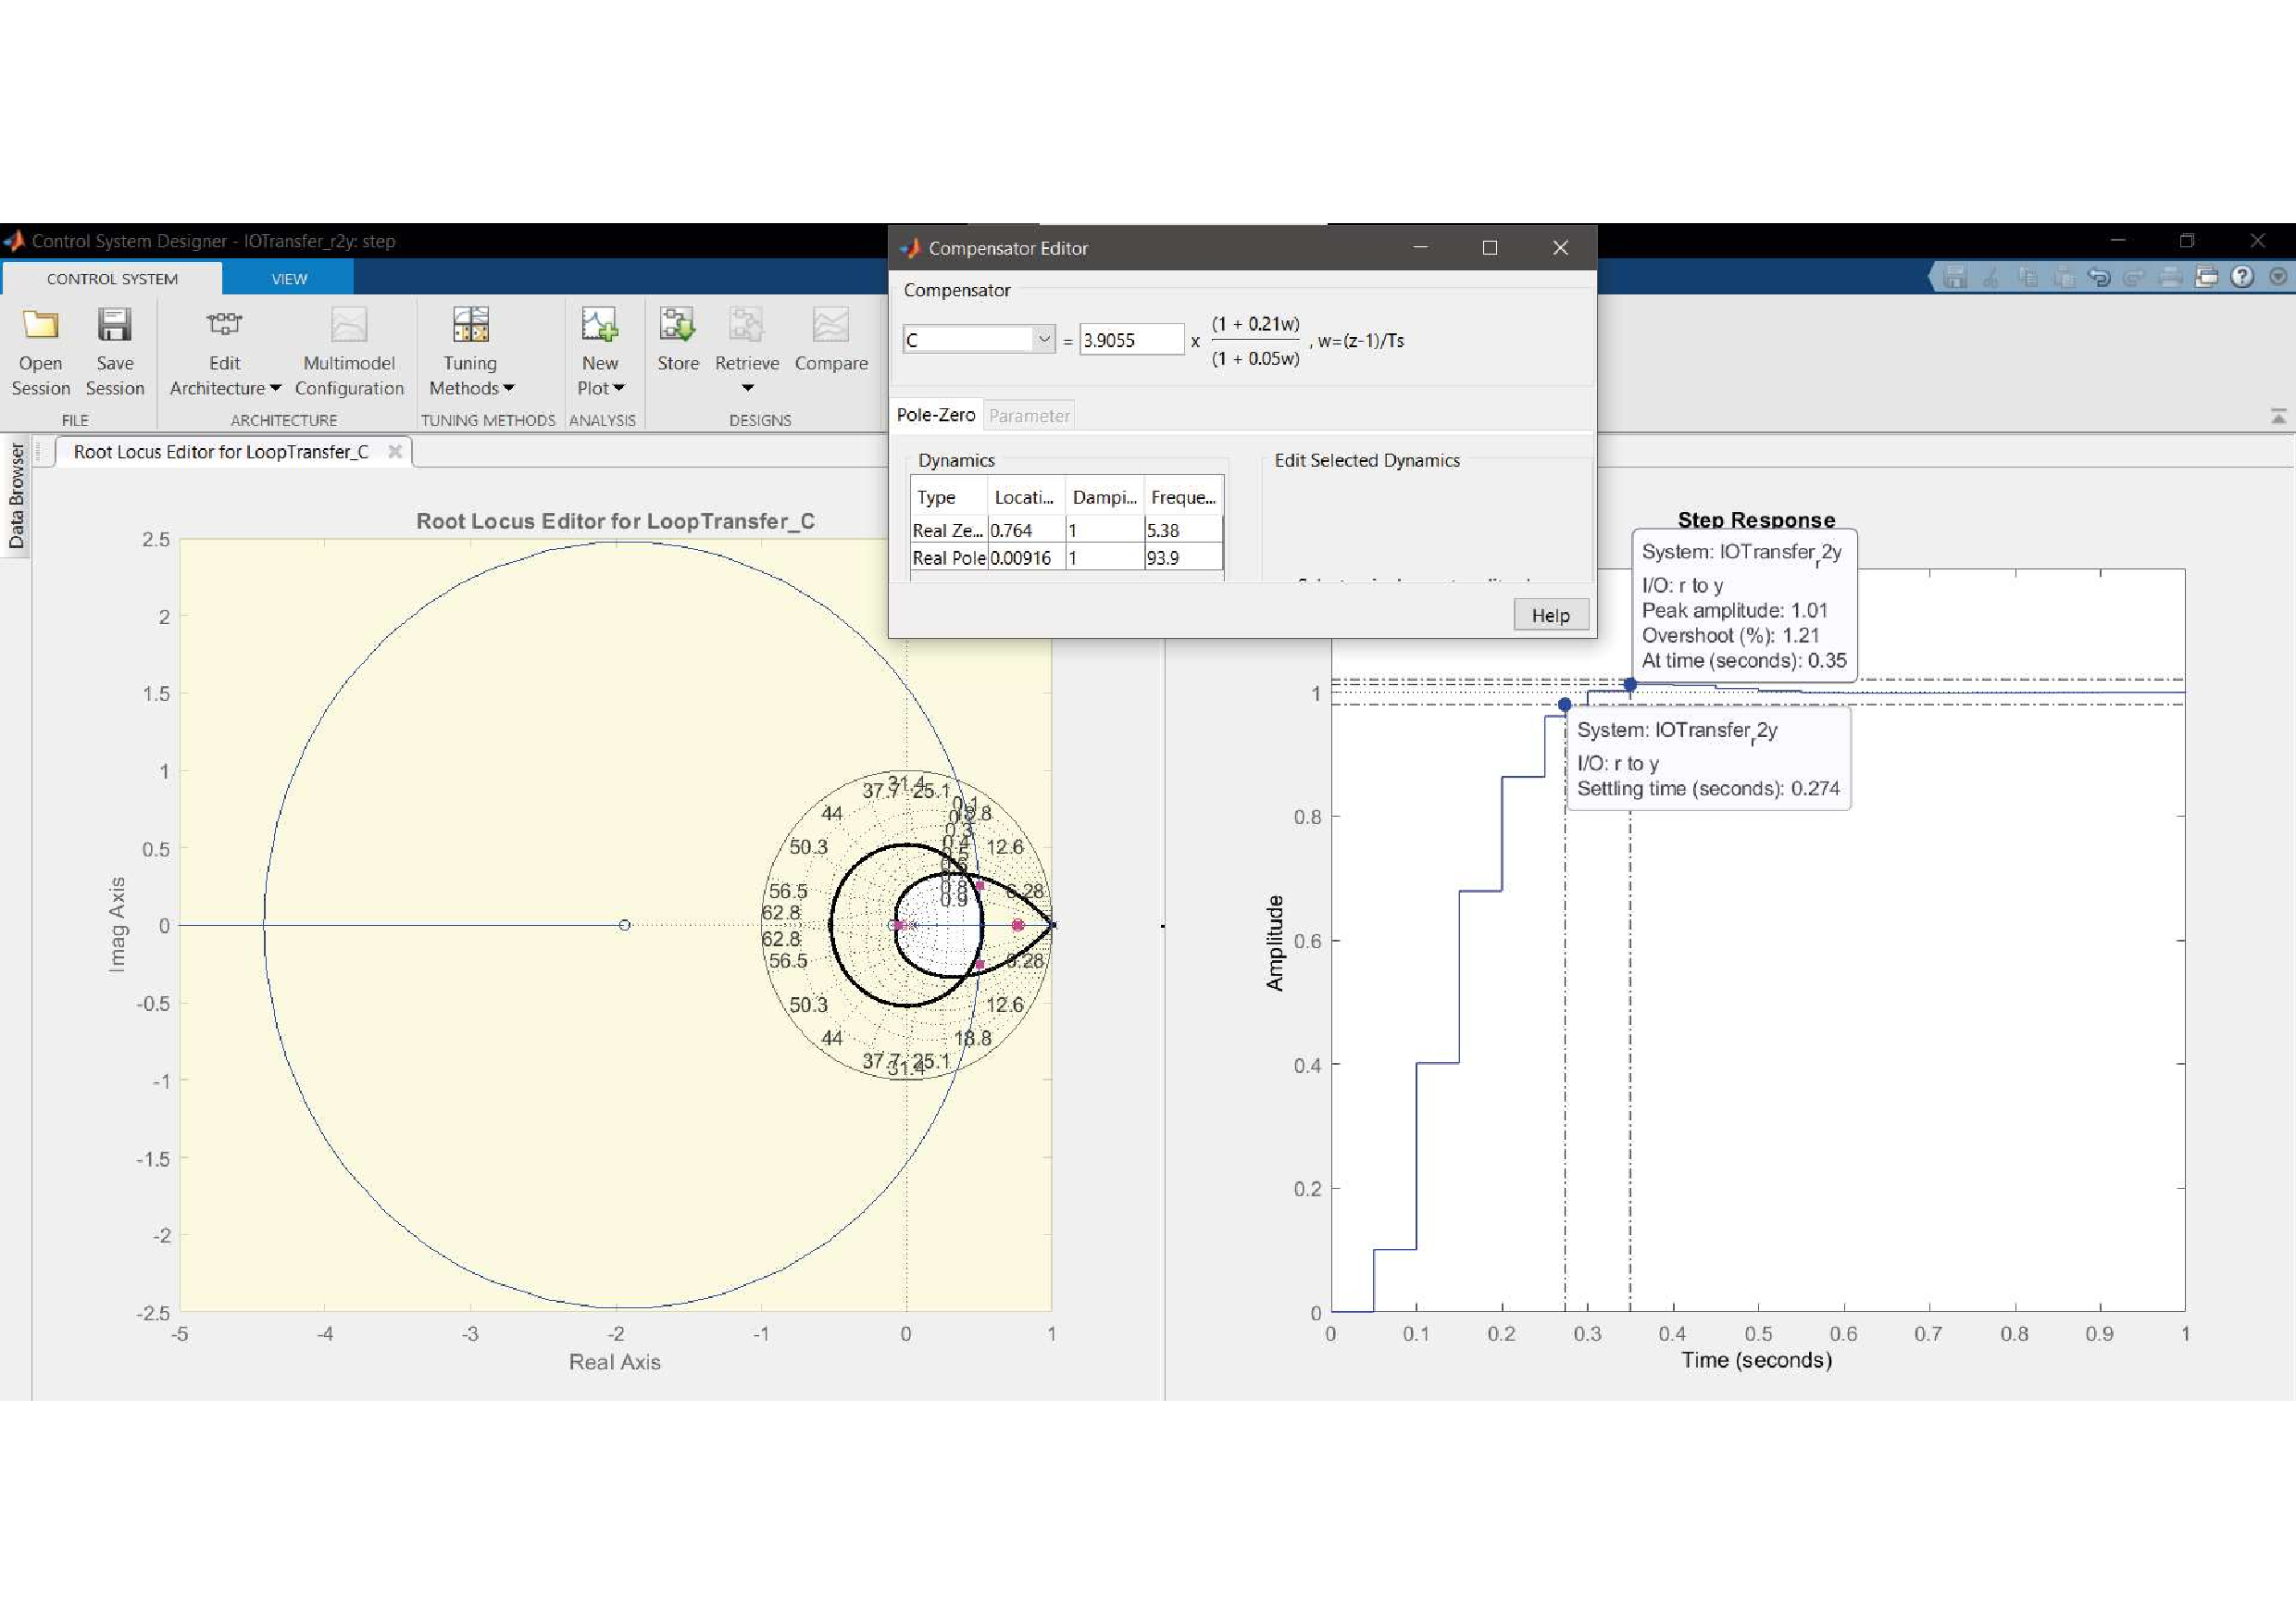
\includegraphics[clip, trim=0cm 4.5cm 0cm 4.2cm,
  scale=0.33]{images/figura 6.pdf}
  % izquierda,abajo,derecha,arriba
  \caption{Controlador PD.}
    \label{fig:figura 6}
\end{figure}
}
\vspace*{0.35em}
Mediante la herramienta \textsc{Export>Export tuned blocks.} podemos
enviar el controlador al espacio de trabajo.

$>>>$ PD\_9
\vspace*{0.35em}
\begin{tcolorbox}[sharp corners, colback = white]
    \color{gray}
\begin{verbatim}
PD_9 =
 
  16.404 (z-0.7641)
  -----------------
    (z-0.009156)
 
Sample time: 0.05 seconds
Discrete-time zero/pole/gain model.
\end{verbatim}
  \end{tcolorbox}%
  \vspace*{0.5em}
\end{tcolorbox}%

\begin{tcolorbox}[sharp corners, colframe=bluebox, title= Respuesta
  del sistema en tiempo discreto con un controlador PD.]
  $>>>$ ltiview(\textcolor{blue}{`step'},kr*feedback(PD\_9*Gposicionz,kr))
  \vspace*{0.35em}
  \mkanscode{
\begin{figure}[H]
  \centering
  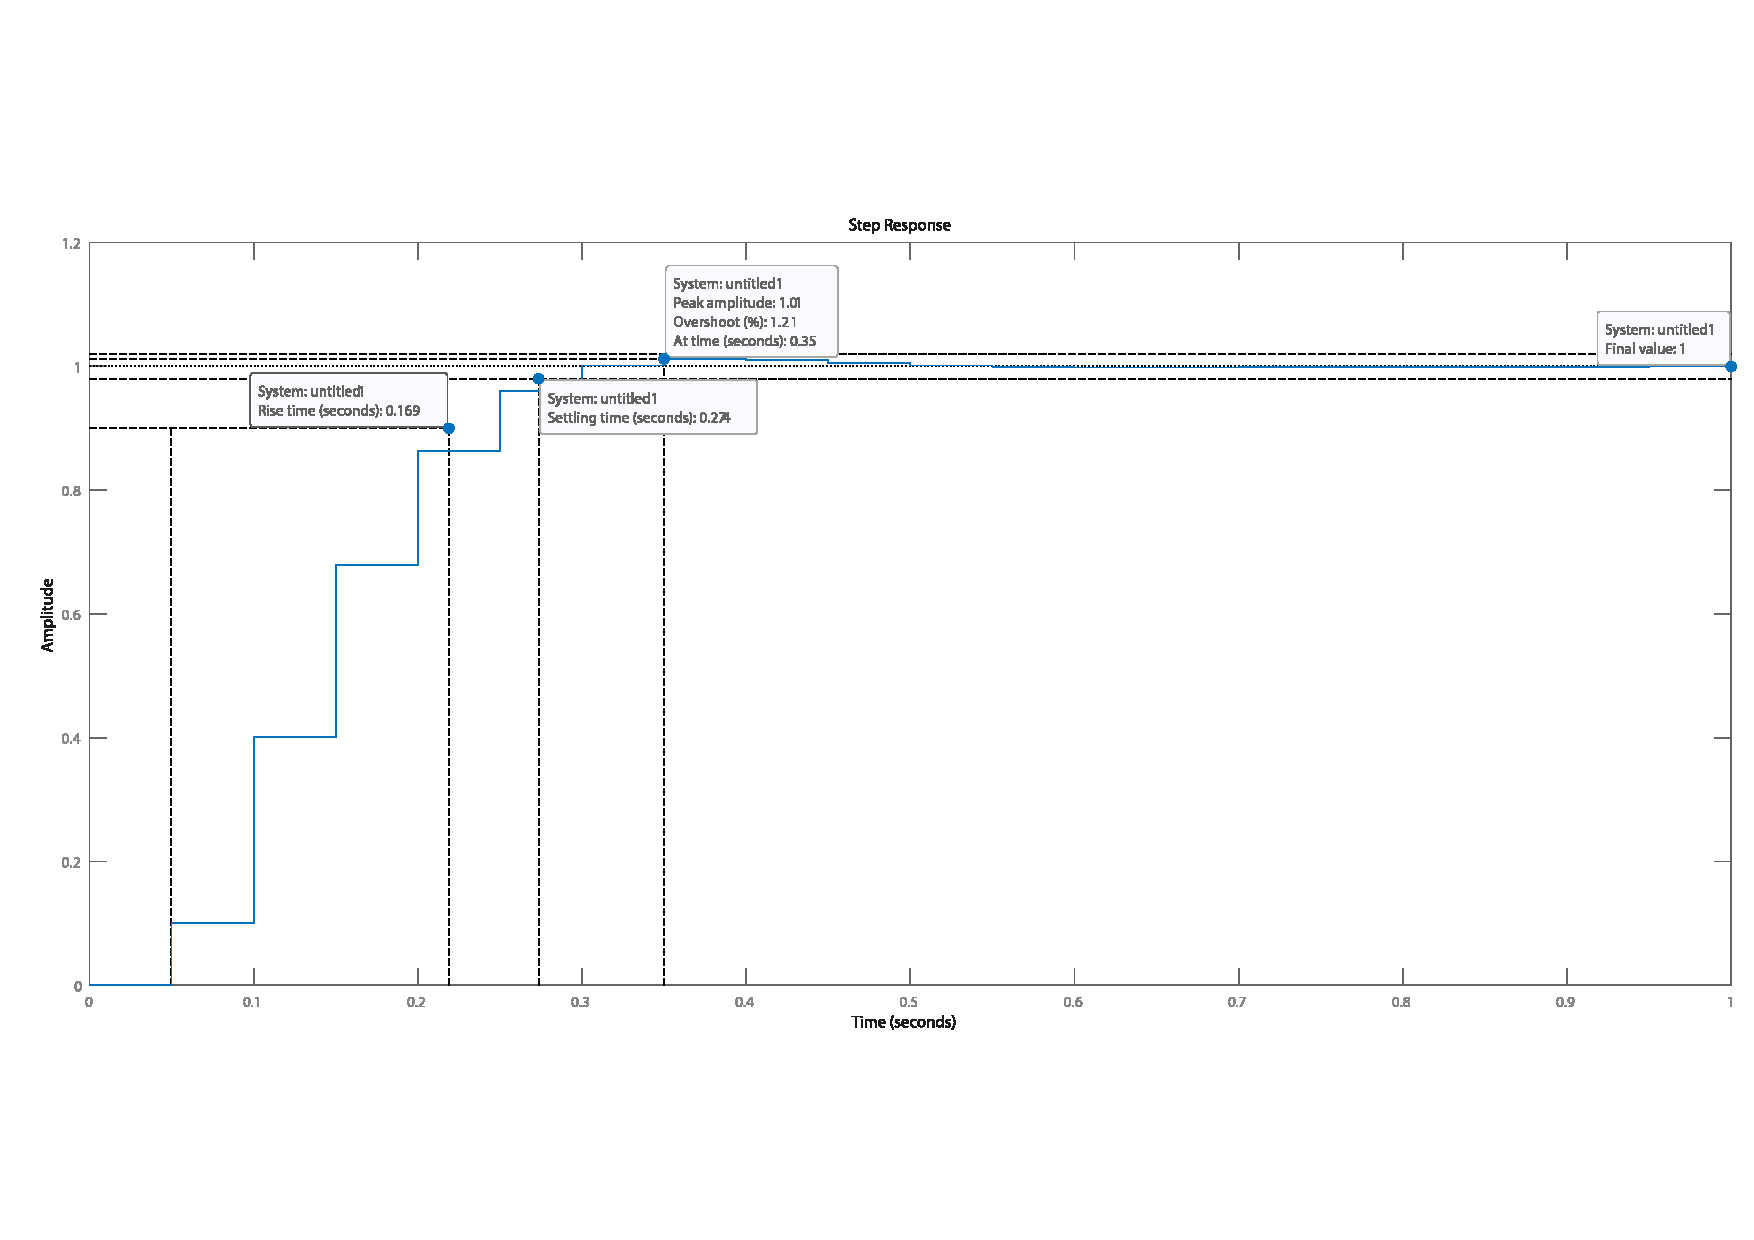
\includegraphics[clip, trim=0cm 3.6cm 0cm 3.7cm,scale=0.40]{images/figura 7.pdf}
  % izquierda,abajo,derecha,arriba
  \caption{Respuesa del sistema frente a un escalón con un controlador PD.}
    \label{fig:figura 7}
\end{figure}
}

\end{tcolorbox}%